% Architecture figure, adapted from the paper's architecture figure.
% Input thumbnail: Liszt, Hungarian Rhapsody No. 2, IMSLP file 300584, page 26 (public domain).
\documentclass[border=6pt]{standalone}
% Shared preamble for the README figures. Compile with build.sh.
\usepackage[T1]{fontenc}
\usepackage[sfdefault,scale=0.95,lining]{FiraSans}
\usepackage[scale=0.9]{sourcecodepro}
\usepackage{textcomp}
\usepackage{graphicx}
\usepackage{xcolor}
\usepackage{tikz}
\usepackage{pgfplots}
\pgfplotsset{compat=1.18}
\usetikzlibrary{arrows.meta,positioning,calc,backgrounds,fit,decorations.pathreplacing}
\graphicspath{{assets/}}
\definecolor{ink}{HTML}{1F2328}
\definecolor{muted}{HTML}{59636E}
\definecolor{rule}{HTML}{D1D9E0}
\definecolor{codebg}{HTML}{F6F8FA}
\definecolor{tc}{HTML}{6F42C1}
\definecolor{tclight}{HTML}{C9B6F2}
\definecolor{legato}{HTML}{F0A35E}
\definecolor{smt}{HTML}{9DB4D6}
\color{ink}

\definecolor{enccolor}{HTML}{4A90D9}
\definecolor{pecolor}{HTML}{5BA85B}
\definecolor{projcolor}{HTML}{888888}
\definecolor{deccolor}{HTML}{E8913A}
\definecolor{sattncolor}{HTML}{D46A4A}
\definecolor{cattncolor}{HTML}{E8913A}
\definecolor{ffncolor}{HTML}{D4A84A}
\definecolor{iocolor}{HTML}{6F42C1}
\definecolor{gramcolor}{HTML}{C04040}
\begin{document}
\begin{tikzpicture}[
    block/.style={draw=#1!70, fill=#1!8, rounded corners=4pt, minimum height=1.8cm, minimum width=2.8cm, font=\small, align=center, line width=0.8pt},
    sublayer/.style={draw=#1!70, fill=#1!15, rounded corners=3pt, minimum height=0.75cm, minimum width=3.4cm, font=\footnotesize, align=center, line width=0.6pt},
    dimlab/.style={font=\footnotesize, text=muted},
    arr/.style={-{Stealth[length=3.5pt, width=2.8pt]}, line width=0.9pt, black!50},
    darr/.style={-{Stealth[length=2.5pt, width=2.2pt]}, line width=0.6pt, black!35},
]
    \node[block=iocolor, minimum width=2.2cm, minimum height=2.4cm] (input) {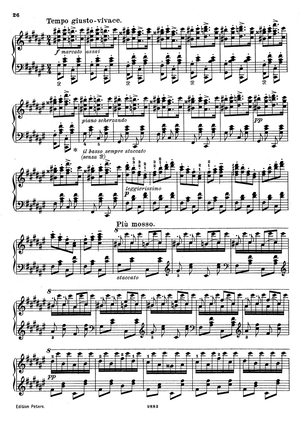
\includegraphics[width=1.7cm]{liszt-p26-thumb.png}};
    \node[dimlab, below=3pt of input] {1485\,\texttimes\,1050 px (fixed)};
    \node[font=\footnotesize, above=3pt of input] {Score image};

    \node[block=enccolor, right=1.0cm of input, minimum width=3.0cm, minimum height=2.4cm]
    (encoder) {\textbf{ConvNeXt-V2}\\[2pt]{\footnotesize pretrained \& finetuned}};
    \node[dimlab, below=3pt of encoder] {46\,\texttimes\,32\,\texttimes\,768};
    \node[font=\footnotesize, text=enccolor!80!black, above=3pt of encoder] {Vision encoder};

    \node[block=projcolor, right=0.8cm of encoder, minimum width=2.6cm, minimum height=2.4cm]
    (proj) {\textbf{Projector MLP}\\[2pt]{\footnotesize Lin.\ \textrightarrow{} GELU \textrightarrow{} Lin.}};
    \node[dimlab, below=3pt of proj] {1472\,\texttimes\,768};

    \node[draw=pecolor!70, fill=pecolor!15, circle, minimum size=0.9cm, font=\normalsize\bfseries, line width=0.8pt, right=1.0cm of proj] (addcircle) {$+$};
    \node[dimlab, below=3pt of addcircle] {1472\,\texttimes\,768};
    \node[block=pecolor, minimum width=2.4cm, minimum height=1.2cm, above=0.8cm of addcircle] (pe) {\textbf{2D Sin.\ PE}};
    \draw[arr, pecolor!60] (pe) -- (addcircle);

    \node[sublayer=sattncolor, right=1.4cm of addcircle, yshift=1.05cm] (selfattn) {\textbf{Self-attention}~~{\footnotesize RoPE}};
    \node[sublayer=cattncolor, below=0.28cm of selfattn] (crossattn) {\textbf{Cross-attention}};
    \node[sublayer=ffncolor, below=0.28cm of crossattn] (ffn) {\textbf{Feed-forward}};

    \coordinate (decoderTop) at ($(selfattn.north)+(0,13pt)$);
    \begin{scope}[on background layer]
        \node[draw=deccolor!40, fill=deccolor!4, rounded corners=5pt, line width=0.9pt, fit=(decoderTop)(selfattn)(crossattn)(ffn), inner xsep=10pt, inner ysep=6pt] (decoder) {};
    \end{scope}
    \draw[decorate, decoration={brace, amplitude=4pt}, line width=0.6pt, black!40]
    ($(decoder.north east)+(3pt,0)$) -- ($(decoder.south east)+(3pt,0)$)
    node[midway, right=6pt, font=\footnotesize] {\texttimes\,10};
    \draw[darr] (selfattn) -- (crossattn);
    \draw[darr] (crossattn) -- (ffn);
    \node[font=\footnotesize, text=deccolor!80!black, above=6pt of selfattn] (toklabel) {Transformer decoder};
    \draw[arr, iocolor!60] (toklabel) -- (selfattn.north);
    \node[dimlab, below=3pt of decoder] {d\textsubscript{model}\,=\,768, 12 heads, d\textsubscript{ff}\,=\,1536};

    \node[draw=gramcolor!70, fill=gramcolor!15, circle, minimum size=0.9cm, font=\normalsize\bfseries, line width=0.8pt, right=1.4cm of decoder.east |- ffn] (maskcircle) {$\otimes$};
    \node[block=gramcolor, minimum width=2.4cm, minimum height=1.2cm, below=0.5cm of maskcircle] (grammar) {\textbf{Constrained}\\\textbf{decoding}};
    \draw[arr, gramcolor!60] (grammar) -- (maskcircle);

    \node[block=iocolor, right=1.3cm of maskcircle, minimum width=2.0cm, minimum height=1.4cm] (output) {\textbf{\texttt{**kern}}\\[2pt]{\footnotesize tokens}};
    \node[dimlab, below=3pt of output] {vocab\,=\,3000};

    \draw[arr] (input) -- (encoder);
    \draw[arr] (encoder) -- (proj);
    \draw[arr] (proj) -- (addcircle);
    \draw[arr] (addcircle) -- (crossattn.west);
    \draw[arr] (ffn.east) -- (maskcircle);
    \draw[arr] (maskcircle) -- (output);

    \coordinate (looptop) at ($(toklabel.north)+(0,0.42cm)$);
    \draw[arr, iocolor!50, rounded corners=5pt]
    (output.north) -- node[font=\footnotesize, right=2pt, pos=0.1] {Output} (output.north |- looptop)
    -- node[font=\footnotesize, text=iocolor!80!black, above=1pt] {autoregressive} (toklabel.north |- looptop)
    -- (decoder.north);
\end{tikzpicture}
\end{document}
